\documentclass{beamer}
\usepackage[absolute,overlay]{textpos}

\setbeamertemplate{bibliography item}[text]
\setbeamertemplate{navigation symbols}{}
\setbeamertemplate{caption}[numbered] 
\setbeamerfont{caption}{size=\scriptsize}

\newcommand\FrameText[1]{
\begin{textblock}{16}(1,2.5)
\raggedright #1
\end{textblock}}

\begin{document}

\addtobeamertemplate{frametitle}{}{
\begin{textblock}{16}(0,0)

\includegraphics[scale=0.5]{Header.png}
\end{textblock}}

\begin{frame}
\frametitle{1}
\begin{picture}(0.0,0.0)
\put(-28.45,-142){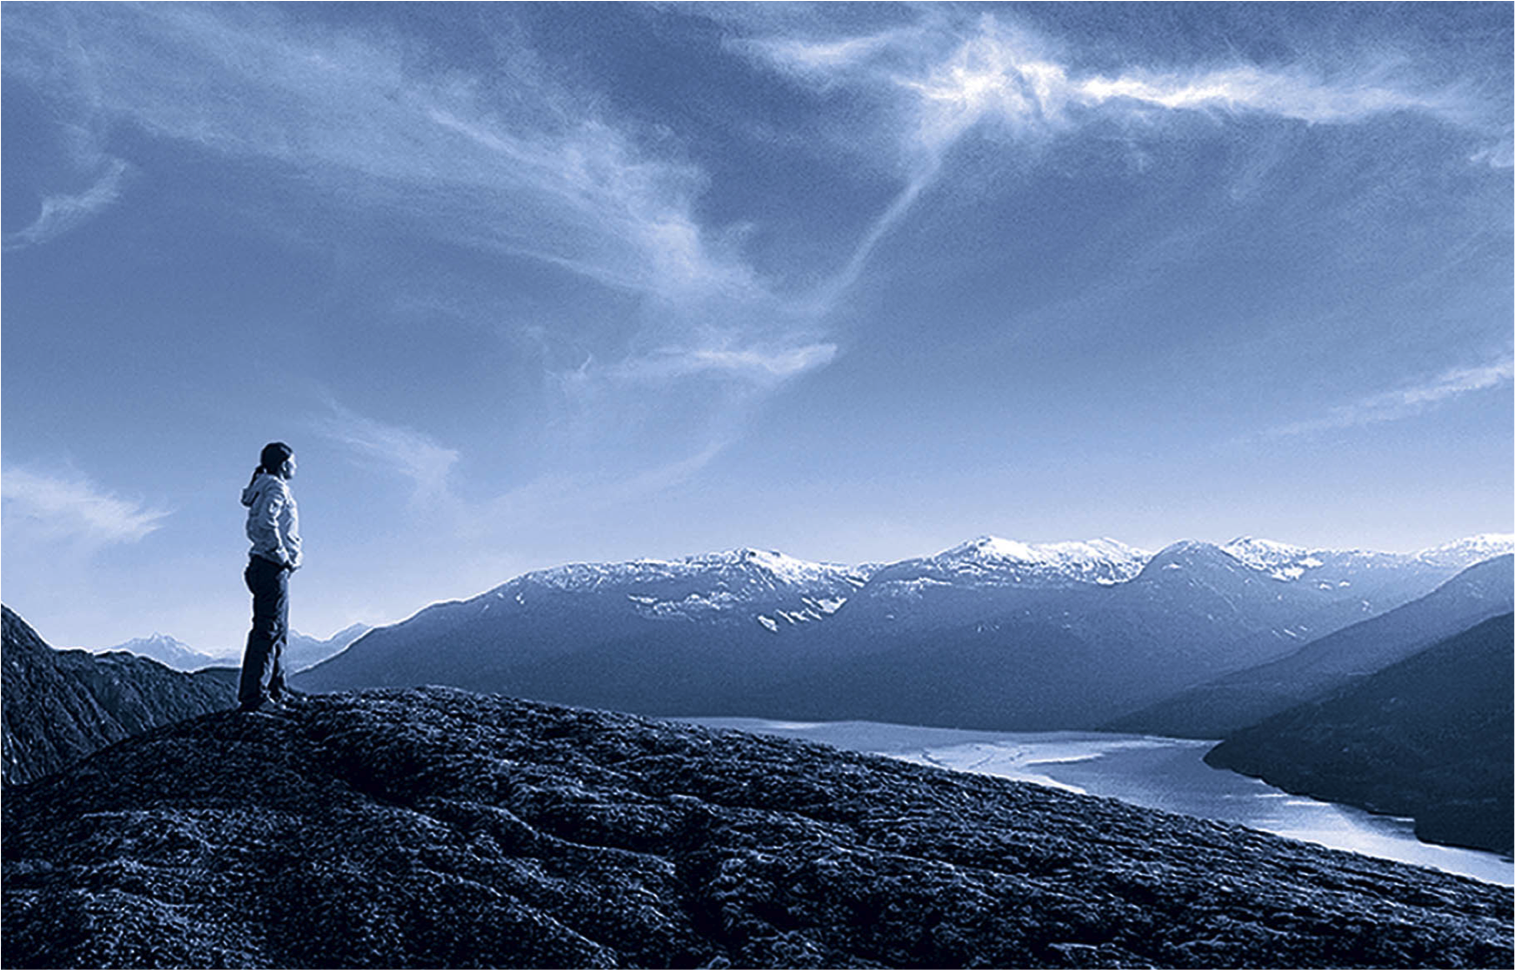
\includegraphics[width=\paperwidth]{FrontPage.png}}
\end{picture}
\FrameText{
\textcolor{white}{\bf{\LARGE }}\\
\textcolor{white}{\bf{\LARGE }}\\
\textcolor{white}{\bf{, MSc , }}}
\end{frame}

\footnotesize

\begin{frame}
\frametitle{2}
\FrameText{\bf{\large}}
\begin{itemize}
\item Principal Component Analysis (PCA) is one of the four main classes of empirical methods used in Oceanography and Atmospheric Science (Hsieh and Tang 1998)~\cite{hsi}
\item An interest in high-latitude climate variability and change - encountered paper on the Influence of the tropics on the Southern Annular Mode (Ding, Steig, Battisti and Wallace 2012)~\cite{din}
\begin{itemize}
\scriptsize
\item[-] Line of investigation relies heavily on PCA
\item[-] Discusses tropical ocean forcings on atmospheric behaviour
\item[-] Recently published, current research
\end{itemize}
\item The result: a two part presentation, focusing on
\begin{itemize}
\scriptsize
\item[-] Mathematical details of the PCA method
\item[-] Discussion of how PCA is used by Ding et. al. to investigate their hypothesis
\end{itemize}
\end{itemize}
\end{frame}

\begin{frame}
\frametitle{3}
\FrameText{\bf{\large Synopsis}}
\begin{itemize}
\item Theoretical Background for Principal Component Analysis
\begin{itemize}
\scriptsize
\normalfont
\item[-] General characteristics and uses of the method
\item[-] An example based, intuitive interpretation of PCA
\item[-] The derivation of the principal components
\item[-] Drawbacks of the method
\end{itemize}
\footnotesize
\item Principal Component Analysis in Ding et. al.
\begin{itemize}
\normalfont
\scriptsize
\item[-] Use of PCA to investigate the hypothesis
\item[-] Findings related to tropically forced variability and superposition of regional patterns in the Southern Annular Mode
\end{itemize}
\end{itemize}
\end{frame}

\begin{frame}
\frametitle{4}
\FrameText{\bf{\large Part 1 -- Theoretical Background for Principal Component Analysis}\\
\footnotesize
\normalfont{following Welch, W. J., 2010: \emph{STAT 306, Finding Relationships in Data:\\
An Introduction to Building Statistical Models}, 8-1 -- 8-8}}
\end{frame}

\begin{frame}
\frametitle{3}
\FrameText{\bf{\large Characteristics of the Method}}

\begin{table}[h]
\begin{center}
\begin{tabular}{|p{5.0cm}|p{5.0cm}|}
\hline
\hline
\textbf{Supervised Learning} (Regression, Logistic Regression) & \textbf{Unsupervised Learning} (PCA, Cluster Analysis)\\
\hline
\hline
Model a response variable as a function of explanatory variables & Search for structure in multivariate data\\
\hline
The response variable is of primary interest & No variable is singled out as a response\\
\hline
Method is supervised in the sense that it is directed toward explaining or predicting this specific variable & Method is
unsupervised in the sense that variables are treated symmetrically in order to understand underlying structure\\
\hline
\end{tabular}
\end{center}
\caption{A Classification of Statistical Methods}
\end{table}
\end{frame}

\begin{frame}
\frametitle{2}
\FrameText{\bf{\large Characteristics of the Method}}
\begin{itemize}
\item Reduces a set of variables to a smaller set
\item Attempts to maintain the total variation in the data
\item It represents a dimension-reduction strategy
\item Often used on large datasets of explanatory variables as pre-processing for another supervised modeling strategy (e.g. Hsieh and Tang 1998)
\end{itemize}
\end{frame}

\begin{frame}
\frametitle{3}
\FrameText{\bf{\large Interpretation as a Transformed Coordinate System}}
\begin{table}[h]
\begin{center}
\begin{tabular}{|p{5.0cm}|p{5.0cm}|}
\hline
\hline
\textbf{Quantity} & \textbf{Notation}\\
\hline
\hline
$p$-dimensional vector of variables describing an observation & $\mathbf{x}=(x_1,...,x_p)^T$ \\
\hline
Dataset with $n$ vectors of variables & $\mathbf{x}^{(1)},...,\mathbf{x}^{(n)}$ \\
\hline
Value of variable $j$ for observation $i$ & $x_j^{(i)}$ \\
\hline
$p$-dimensional vector of sample means for the $n$ observations & $\mathbf{\overline{x}}=(\overline{x}_1,...,\overline{x}_p)$ \\
\hline
$p*p$ sample covariance matrix & $\mathbf{S}$ \\
\hline
Sample mean & $\overline{x}_j=\frac{1}{n}\sum\limits_{i=1}^n x_j^{(i)}\;\;(j=1,...,p)$ \\
\hline
Sample covariance matrix & $\mathbf{S}_{jj'}=\frac{1}{n-1}\sum\limits_{i=1}^n(x_j^{(i)}-\overline{x}_j)(x_{j'}^{(i)}-\overline{x}_{j'})~(j=1,...,p,j'=1,...,p)$\\
\hline
\end{tabular}
\end{center}
\caption{Formal Notation}
\end{table}
\end{frame}

\begin{frame}
\frametitle{2}
\FrameText{\bf{\large Interpretation as a Transformed Coordinate System}}
\begin{itemize}
\item For data on $p$ variables $\mathbf{x}=(x_1,...,x_p)^T$, the aim is to identify an orthogonal subspace of dimension $p'<p$ containing most of the variability in the data
\item This subspace will contain $p'$ variables
\item The new variables form a new orthogonal coordinate system and are called principal components (PC)
\item The orthogonal subspace of $p-p'$ variables will contain little variability
\item PCA is generally applied to high-dimensional data, but a 2-dimensional example illustrates the method
\end{itemize}
\end{frame}

\begin{frame}
\frametitle{2}
\FrameText{\bf{\large Interpretation as a Transformed Coordinate System}}
\begin{figure}
\centering
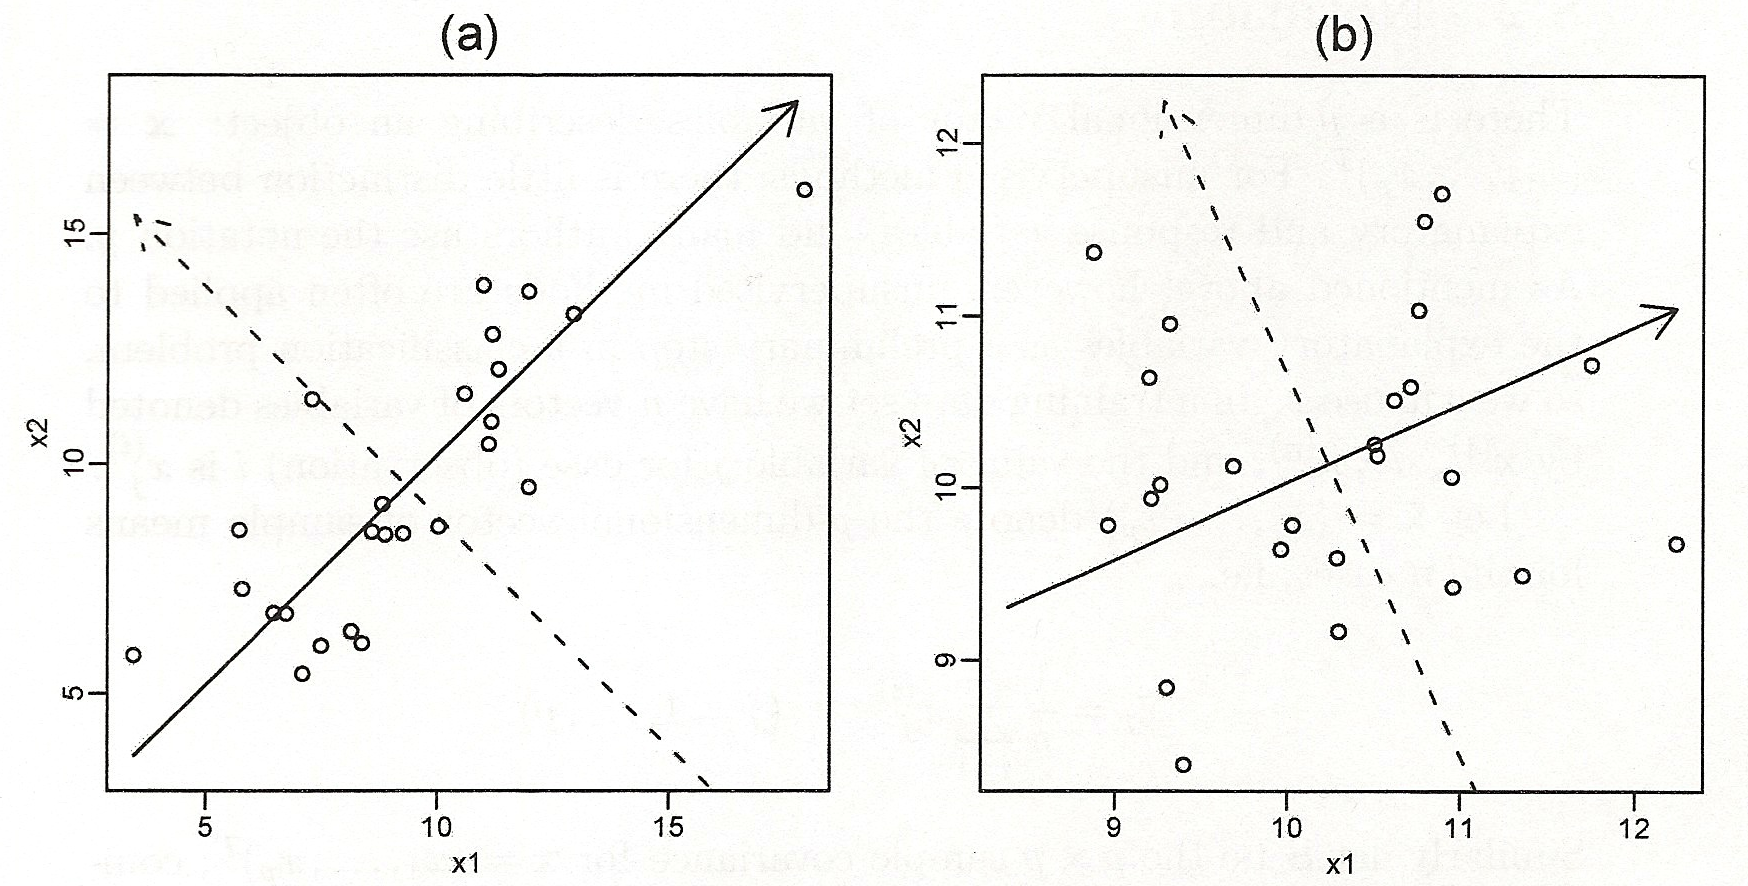
\includegraphics[width=8cm]{2DPCA.png}
\caption{Principal components as a transformed coordinate system; first PC shown by solid line, second PC shown by dashed line. (a) Highly correlated data (b) Approximately uncorrelated data}
\label{PCAExample}
\end{figure}
\end{frame}

\begin{frame}
\frametitle{2}
\FrameText{\bf{\large Interpretation as a Transformed Coordinate System}}
\begin{itemize}
\item Figure~\ref{PCAExample}(a) illustrates a transformation from the initial coordinate system $x_1,...,x_p$ to a new orthogonal coordinate system $v_1,...,v_p$
\item In Figure~\ref{PCAExample}(a), only $p'$ PCs were needed to approximate the space spanned by $x_1,...,x_p$; this is when the PCA method is useful
\item In formal terms, PC $j$ is defined as a linear combination
  of $x_1,...,x_p$ using weights
  $\mathbf{w}^{(j)}=(w_1^{(j)},...,w_p^{(j)})^T$:
\begin{equation}
v_j=w_1^{(j)}x_1+...+w_p^{(j)}x_p=\mathbf{w}^{{(j)}^T}\mathbf{x}
\end{equation}                       
\end{itemize}
\end{frame}

\begin{frame}
\frametitle{2}
\FrameText{\bf{\large Derivation of Principal Components}}
\begin{itemize}
\item Let $\mathbf{w}^{(1)}$ be the coefficient vector of the
  first PC $v_1=\mathbf{w}^{(1)^{T}}\mathbf{x}$, chosen to maximize
  the variance of $v_1$ (i.e. capture as much of the variability in
  $x_1,...,x_p$ as possible)
\item The variance of the first PC can be written as
\begin{equation}
Var(v_1)=Var(\mathbf{w}^{(1)^{T}}\mathbf{x})=\mathbf{w}^{(1)^{T}}\mathbf{S}\mathbf{w}^{(1)}
\end{equation}
\item We seek to maximize the variance
\begin{equation}
max_{\mathbf{w}^{(1)}}\;\;\mathbf{w}^{(1)^{T}}\mathbf{S}\mathbf{w}^{(1)}
\end{equation}
\item Vector $w$ must be constrained to have unit length
\begin{equation}
\mathbf{w}^{(1)^{T}}\mathbf{w}^{(1)}=1
\end{equation}
\end{itemize}
\end{frame}

\begin{frame}
\frametitle{2}
\FrameText{\bf{\large Derivation of Principal Components}}
\begin{itemize}
\item Maximization under a constraint requires the technique of Lagrange multipliers
\begin{equation}
max_{\mathbf{w}^{(1)},\lambda_1}\;\;\mathbf{w}^{(1)^{T}}\mathbf{S}\mathbf{w}^{(1)}-\lambda_1(\mathbf{w}^{(1)^{T}}\mathbf{w}^{(1)}-1)
\label{eq1}
\end{equation}
\item Differentiating with respect to $w$ results in $p$ equations
\begin{equation}
2\mathbf{Sw}^{(1)}-2\lambda_1\mathbf{w}^{(1)}=0
\end{equation}
\begin{equation}
\mathbf{Sw}^{(1)}=\lambda_1\mathbf{w}^{(1)}
\label{eq}
\end{equation}
\item $\lambda_1$ is an eigenvalue of $\mathbf{S}$ and $w_1$ is an eigenvector of $\mathbf{S}$
\end{itemize}
\end{frame}

\begin{frame}
\frametitle{2}
\FrameText{\bf{\large Derivation of Principal Components}}
\begin{itemize}
\item Moreover, $w_1$ is a normalized eigenvector of $\mathbf{S}$, as differentiating (\ref{eq1}) with respect to $\lambda$ yields the original constraint
\begin{equation}
-(\mathbf{w}^{(1)^{T}}\mathbf{w}^{(1)}-1)=0
\end{equation}
\begin{equation}
\mathbf{w}^{(1)^{T}}\mathbf{w}^{(1)}=1
\end{equation}
\item The maximum value of the variance is obtained by pre-multiplying both sides of (\ref{eq}) by $\mathbf{w}^{(1)^{T}}$
\begin{equation}
\mathbf{w}^{(1)^{T}}\mathbf{Sw}^{(1)}=\lambda_1\mathbf{w}^{(1)^{T}}\mathbf{w}^{(1)}=\lambda_1
\end{equation}
\item $Var(v_1)$ is maximized if $\lambda_1$ is the maximum eigenvalue of $\mathbf{S}$ and the corresponding eigenvector is the first PC
\end{itemize}
\end{frame}

\begin{frame}
\frametitle{2}
\FrameText{\bf{\large Derivation of Principal Components}}
\begin{itemize}
\item Remaining PCs are determined using a similar method, with the additional constraints that arise because of orthogonality to the previously determined PCs
\begin{equation}
v_2=\mathbf{w}^{(2)^{T}}\mathbf{x}
\end{equation}
\begin{equation}
Var(v_2)=\mathbf{w}^{(2)^{T}}\mathbf{S}\mathbf{w}^{(2)}
\end{equation}
\item Subject to the constraints
\begin{equation}
\mathbf{w}^{(2)^{T}}\mathbf{w}^{(2)}=1
\end{equation}
\begin{equation}
\mathbf{w}^{(1)^{T}}\mathbf{w}^{(2)}=0
\end{equation}
\item This results in the maximum variance that is orthogonal to the first PC
\end{itemize}
\end{frame}

\begin{frame}
\frametitle{2}
\FrameText{\bf{\large Derivation of Principal Components}}
\begin{itemize}
\item After all PCs are determined via a similar method, the following relationships are true
\begin{equation}
\lambda_1\geq...\geq\lambda_p
\end{equation}
\begin{equation}
Var(v_1)\geq...\geq Var(v_p)
\end{equation}
\begin{equation}
\sum\limits_{j=1}^p Var(v_j)=\sum\limits_{j=1}^p\lambda_j=\sum\limits_{j=1}^p Var(x_j)
\end{equation}
\item The percentage of the total variability captured in the lower-dimensional subspace depends on the number of PCs retained
\item PCA is thus a dimension-reduction strategy which attempts to maintain the total variation in the data
\end{itemize}
\end{frame}

\begin{frame}
\frametitle{2}
\FrameText{\bf{\large Drawbacks of Principal Component Analysis}}
\begin{itemize}
\item Scaling -- PCA is not scale invariant; the determined PCs will be biased towards large variables. Variables must be scaled to have the same units and similar ranges. Alternatively the correlation matrix can be used instead of the covariance matrix.
\item Relevance to Subsequent Analysis -- potentially important information has been discarded
\item Linearity -- PCA does not help uncover non-linear relationships between the variables
\end{itemize}
\end{frame}

\begin{frame}[fragile]
\frametitle{2}
\FrameText{\bf{\large Practical Implementation of PCA}}
\begin{itemize}
\item PCA is available in powerful software packages, such as the statistical package R
\item The input below is sufficient to perform PCA of a simple dataset
\tiny{\begin{verbatim}
bankrupt=read.table("bankruptcytrain.txt",header=TRUE,skip=5)
attach(bankrupt)
pca=princomp(bankrupt[,-5],cor=TRUE,scores=T)
summary(pca)
\end{verbatim}}
\footnotesize
\item The resulting output is shown below
\tiny{\begin{verbatim}
Importance of components:
                         Comp.1    Comp.2    Comp.3     Comp.4
Standard deviation     1.528140 1.0312955 0.6901442 0.35343839
Proportion of Variance 0.583803 0.2658926 0.1190748 0.03122967
Cumulative Proportion  0.583803 0.8496956 0.9687703 1.00000000
\end{verbatim}}
\end{itemize}
\end{frame}

\begin{frame}
\frametitle{1}
\FrameText{
\bf{\large Part 2 -- Principal Component Analysis in}\\
\bf{\large  Ding et. al.}\\
\normalfont{following Ding, Q., Steig, E.J., Battisti, D.S., and Wallace J.M., 2012:\\
\emph{Influence of the tropics on the Southern Annular Mode}. J. Climate, 25, 6330-48.}}
\end{frame}

\begin{frame}
\frametitle{2}
\FrameText{\bf{\large What is the Southern Annular Mode?}}
\begin{itemize}
\item The dominant PC of the Southern Hemisphere (SH) atmospheric circulation
\item Accounts for 20\%-30\% of the monthly sea level pressure (SLP) or geopotential height variability south of $20^{\circ}$S
\item Usually defined from the sea level pressure or lower troposphere geopotential height fields in the SH
\item Ding et. al. 2010~\cite{din} use the 200-hPa geopotential heights $Z_{200}$ because they are at the core of the tropospheric jetstream and can potentially capture the greatest circulation variance
\item The time varying SAM index is defined as the projection of SLP or geopotential anomalies onto this PC
\item It is widely accepted to exist due to internal atmospheric dynamics
\end{itemize}
\end{frame}

\begin{frame}
\frametitle{2}
\FrameText{\bf{\large Influence of the Tropics on the Southern Annular
  Mode}}
\begin{itemize}
\item Presents evidence that perturbations in the southern
  annular mode (SAM) are correlated with sea surface temperature (SST)
  anomalies in the tropical Pacific
\item SAM variability is found to be zonally asymmetric for the
  Eastern and Western Hemispheres
\begin{itemize}
\scriptsize
\item[-] Internal dynamics are found to prevail in the Indian Ocean sector
\item[-] Forced response to SST anomalies influences the Pacific Ocean sector
\end{itemize}
\end{itemize}
\end{frame}

\begin{frame}
\frametitle{2}
\FrameText{\bf{\large Focus of the Research}}
\begin{itemize}
\item Test hypothesis that the SAM is not entirely an intrinsic feature of high-latitude atmospheric dynamics
\item Investigate whether SAM may include variability that is tropically forced
\item Investigate whether SAM may be a superposition of regional patterns
\item Investigate epochal differences in the SH circulation (not discussed here)
\item Provide a dynamical interpretation of the findings (not discussed here)
\end{itemize}
\end{frame}

\begin{frame}
\frametitle{2}
\FrameText{\bf{\large Canonical SAM Pattern at 200 hPa}}
\begin{itemize}
\item Monthly and seasonal mean plots of the variability of
  $Z_{200}$ anomalies shown in Figures~\ref{1} and~\ref{2} reveal maximum
  variability over West Antarctica and the Amundsen Sea (AS, ``pole of variability'')
\item The PC associated with the first Empirical Orthogonal
  Function (EOF) or EOF1 (defined above as the SAM index) is highly
  correlated with other commonly used indices
\item It explains 21\% of the month-to-month variance south of
  $20^{\circ}$S and is well separated from the remaining eigenvectors
\item Region of strongest loading for EOF1 is over the AS and
  coincides with the region of largest month-to-month variability, as
  shown in Figure~\ref{3} 
\end{itemize}
\end{frame}

\begin{frame}
\frametitle{2}
\FrameText{\bf{\large Canonical SAM Pattern at 200 hPa}}
\begin{figure}
\centering
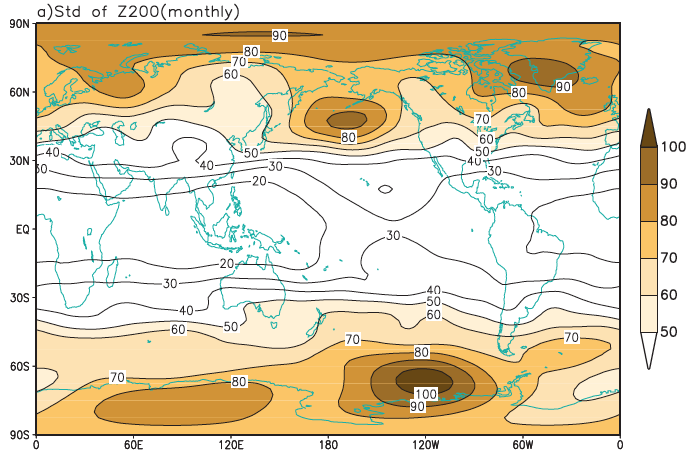
\includegraphics[width=7cm]{1.png}
\caption{\tiny Standard deviation of 200-hPa geopotential height $Z_{200}$ anomalies, 1979-2009 (ECMWF reanalysis data)
for (a) monthly mean for all calendar months}
\label{1}
\end{figure}
\end{frame}

\begin{frame}
\frametitle{2}
\FrameText{\bf{\large Canonical SAM Pattern at 200 hPa}}
\begin{figure}
\centering
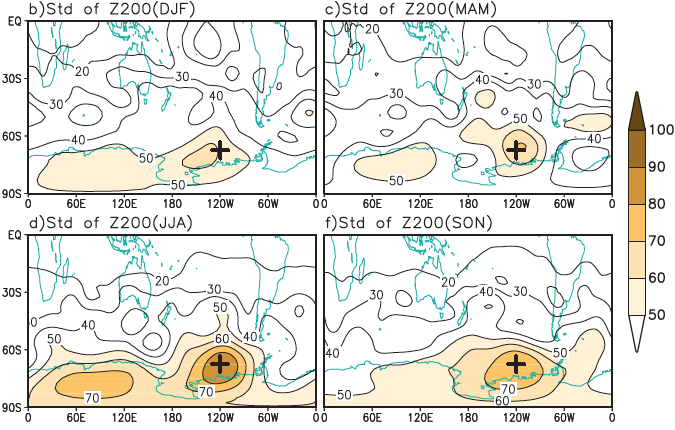
\includegraphics[width=7cm]{2.png}
\caption{\tiny Standard deviation of 200-hPa geopotential height $Z_{200}$ anomalies, 1979-2009 (ECMWF reanalysis data)
for (b) DJF seasonal mean, (c) MAM seasonal mean, (d) JJA seasonal
mean, and (e) SON seasonal mean (contour interval 10 m). Cross denote the location ($67.5^{\circ}$S,$120^{\circ}$W defined as the
AS point hereafter) in the Amundsen Sea, where the variability of $Z_{200}$ is the largest in the SH in most seasons.}
\label{2}
\end{figure}
\end{frame}

\begin{frame}
\frametitle{2}
\FrameText{\bf{\large Canonical SAM Pattern at 200 hPa}}
\begin{figure}
\centering
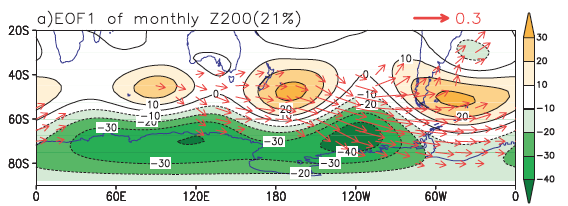
\includegraphics[width=7cm]{3.png}
\caption{\tiny EOF1 of 31-yr (1979-2009) monthly-mean SH 200-hPa height anomalies based on data
for all calendar months (contour interval 10 m). EOF1, explaining 21\%
of total variance, has been scaled by one standard deviation of the corresponding principal component.}
\label{3}
\end{figure}
\end{frame}

\begin{frame}
\frametitle{2}
\FrameText{\bf{\large Seasonality of the SAM and Correlation with Tropical SST}}
\begin{itemize}
\item The correlations of the SAM index with the monthly and seasonal SST anomalies suggest a linkage between the SAM index and a tropical forcing, as shown in Figure~\ref{4} 
\item Figure~\ref{5} shows significant correlations occur during the Austral winter (JJA) between the SAM index and the SST variability in the western-central Pacific and in the Austral summer (DJF) in the eastern Pacific
\end{itemize}
\end{frame}

\begin{frame}
\frametitle{2}
\FrameText{\bf{\large Seasonality of the SAM and Correlation
with Tropical SST}}
\begin{figure}
\centering
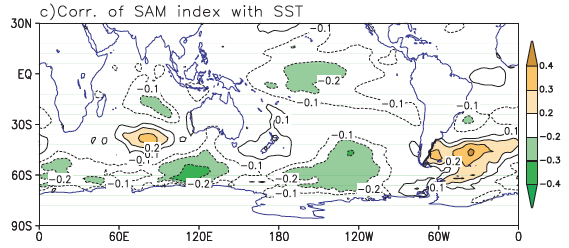
\includegraphics[width=7cm]{4.png}
\caption{\tiny Correlation between PC1 and global monthly-mean SST for the period 1979-2009.
Significant correlations above 99\% confidence level are highlighted by shading.}
\label{4}
\end{figure}
\end{frame}

\begin{frame}
\frametitle{2}
\FrameText{\bf{\large Seasonality of the SAM and Correlation
with Tropical SST}}
\begin{figure}
\centering
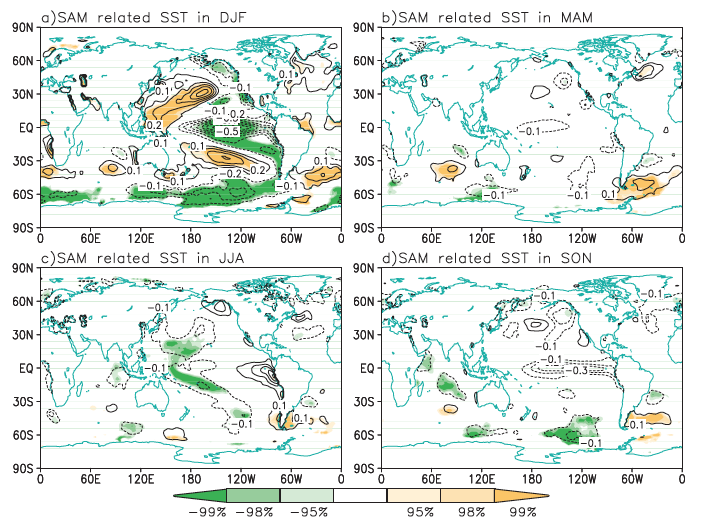
\includegraphics[width=7cm]{5.png}
\caption{\tiny Regression of the seasonal mean SAM index against
  seasonal mean SST anomalies (contour interval $0.1^{\circ}$ C)
for (a) DJF, (b) MAM, (c) JJA, and (d) DJF. Shading denotes regions in which correlation is significant at or above
the 95\% confidence level.}
\label{5}
\end{figure}
\end{frame}

\begin{frame}
\frametitle{2}
\FrameText{\bf{\large Seasonality of the SAM and Correlation with Tropical SST}}
\begin{itemize}
\item The region high variability in the Amundsen Sea identified previously
  exhibits strong loading, suggesting as a next step in the
  investigation a one-point regression between the Amundsen Sea (point AS) and SH $Z_{200}$ and
  SST anomalies
\item These are illustrated in Figure~\ref{6} and strongly
  resemble the corresponding seasonal maps for the leading EOF
\item This is further supported by the correlation between SST anomalies in the
  boxed regions and SLP, as illustrated in Figure~\ref{7} 
\item This evidence suggests that the EOFs are dominated by the
  circulation variability over the Amundsen Sea
\end{itemize}
\end{frame}

\begin{frame}
\frametitle{2}
\FrameText{\bf{\large Seasonality of the SAM and Correlation
with Tropical SST}}
\begin{figure}
\centering
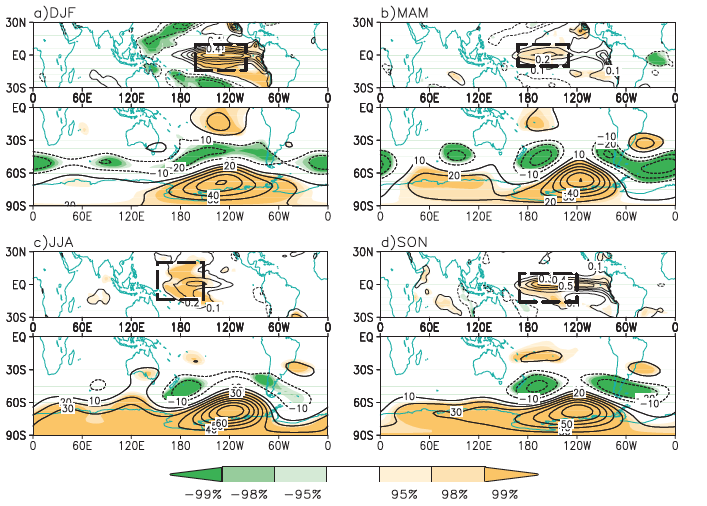
\includegraphics[width=7cm]{6.png}
\caption{\tiny Regression of $Z_{200}$ over the AS point
  ($67.5^{\circ}$S, $120^{\circ}$W) in the Amundsen Sea against (top)
  tropical SST (contour interval $0.1^{\circ}$C) and (bottom) SH $Z_{200}$ (contour interval 10 m) for (a) DJF, (b) MAM, (c) JJA, and (d) DJF.
Shading denotes regions in which correlation is significant at or above the 95\% confidence level.}
\label{6}
\end{figure}
\end{frame}

\begin{frame}
\frametitle{2}
\FrameText{\bf{\large Seasonality of the SAM and Correlation
with Tropical SST}}
\begin{figure}
\centering
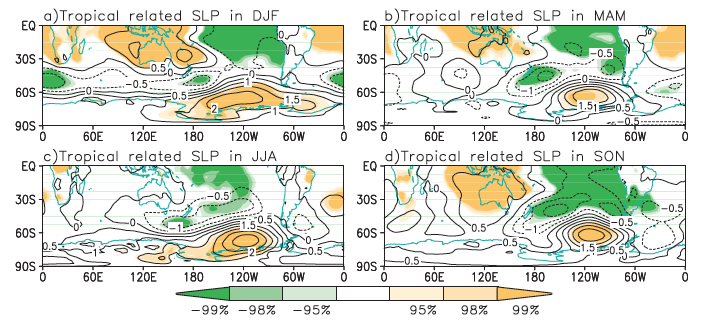
\includegraphics[width=7cm]{7.png}
\caption{\tiny Regression of tropical SST over the key region (denoted by box in the corresponding season)
against SH SLP anomalies (contour interval 0.5 hPa) for (a) DJF, (b) MAM, (c) JJA, and (d) DJF. Shading denotes
regions in which correlation is significant at or above the 95\% confidence level.}
\label{7}
\end{figure}
\end{frame}

\begin{frame}
\frametitle{2}
\FrameText{\bf{\large Decomposition of the SAM into Regional Patterns}}
\begin{itemize}
\item To examine whether the SAM may represent a superposition
  of regional patterns, the variability component associated with the
  Amundsen Sea variability is removed
\item This procedure removes an average of 13\% of the total
  variability south of $20^{\circ}$S
\item EOF1 of the residual monthly data exhibits a zonal dipole
  pattern, which is specific to the Eastern Hemisphere, as illustrated
  in Figure~\ref{8}
\item Finally, the correlation between the seasonal-mean index of
the EOF1 of the residual data and simultaneous SST anomalies shown in
Figure~\ref{9} suggests this regional index is related to SST
anomalies in JJA and SON
\end{itemize}
\end{frame}

\begin{frame}
\frametitle{2}
\FrameText{\bf{\large Decomposition of the SAM into Regional Patterns}}
\begin{figure}
\centering
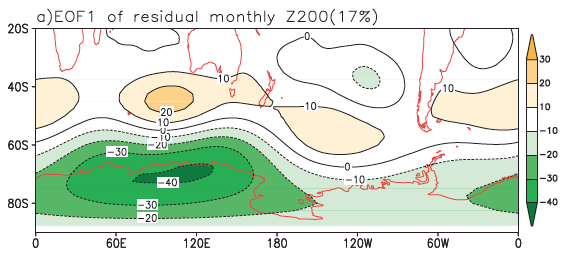
\includegraphics[width=7cm]{8.png}
\caption{\tiny EOF1 of 31-yr (1979-2009) residual monthly mean SH 200 hPa height anomalies
(contour interval 10m). EOF1 has been scaled by one standard deviation of the corresponding
principal component.}
\label{8}
\end{figure}
\end{frame}

\begin{frame}
\frametitle{2}
\FrameText{\bf{\large Decomposition of the SAM into Regional Patterns}}
\begin{figure}
\centering
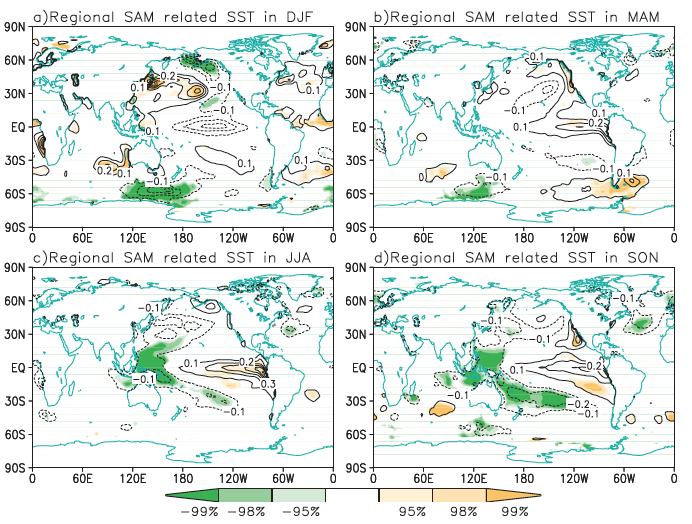
\includegraphics[width=7cm]{9.png}
\caption{\tiny Regression of seasonal mean PC1 of residual monthly mean SH 200-hPa height anomalies against
seasonal mean SST anomalies (contour interval $0.1^{\circ}$C) for (a) DJF, (b) MAM, (c) JJA, and (d) DJF. Shading denotes
regions in which correlation is significant at or above the 95\% confidence level.}
\label{9}
\end{figure}
\end{frame}

\begin{frame}
\frametitle{2}
\FrameText{\bf{\large Summary}}
\begin{itemize}
\item Reviewed an intuitive interpretation of the unsupervised learning technique of PCA as a transformed coordinate system
\item Showed that PCA is a dimension reduction strategy using a simple 2-dimensional example
\item Worked through the mathematical derivation of the principal components
\item Reviewed the work of Ding et. al.~\cite{din} where the SAM (SH EOF1) is correlated to tropical SST anomalies to test the hypothesis that SAM is not entirely an intrinsic feature of high-latitude atmospheric dynamics
\item Ding et. al.~\cite{din} also identified a possible superposition of regional patterns in the SAM by eliminating the dominant EOF
\end{itemize}
\end{frame}

\begin{frame}
\frametitle{2}
\FrameText{\bf{\large References}}
\begin{thebibliography}{99}
\bibitem{din}Ding, Q., Steig, E.J., Battisti, D.S., and Wallace J.M., 2012: \emph{Influence of the tropics on the Southern Annular Mode}. J. Climate, 25, 6330-48.
\bibitem{hsi}Hsieh, W. W., and B. Y. Tang, 1998: \emph{Applying neural network models to prediction and data analysis in meteorology and oceanography}. Bulletin of the American Meteorological Society, 79.
\bibitem{wel}Welch, W. J., 2010: \emph{STAT 306, Finding Relationships in Data: An Introduction to Building Statistical Models}, 8-1 -- 8-8.
\end{thebibliography}
\end{frame}

\end{document}


